\chapter{Experimental Setup}
\label{sec:setup}
	In our experiment, we are detecting, mostly cosmic muons slowed by iron block(26 cm thick), using three layers of plastic scintillators (P0, P1 and P2) coupled to photo multipliers tubes (PMTs) each via a light guide. Due to the mechanisms of energy loss, from Bethe-Bloch formula, the minimum energy needed by muons to pass through 26 cm of iron is $E_{\mu} \approx 382 MeV$ (considering muons at the minimum of ionization energy). Moreover, the block of iron reduces the electromagnetic component of the cosmic rays.
	The incoming muons are detected by the counters P0 and P1 which are thin enough to allow the muons to pass through. During the passage, these charged muons excite the vibrational motion of the molecules which, when de-energized, emit visible light photons( ~1 photon for every 100 eV deposited). The number of photons produced by scintillation is proportional (within statistical considerations) to the energy loss of the passing particle. Those photons will enter the PMT and produce electrons that form the electrical pulse we measure. The size of electronic pulse in a PMTs is proportional to the number of photons produced by scintillator. To maximize the numbers of photon that reach the photocathode of the PMTs, it is necessary that the scintillator, light guide and photomultiplier tube all be wrapped in reflective foil. Also, to block external light the assembly is then covered by black tape.
	After P1, the muons encounter a slab of iron in which some of them eventually stop and decay. If it happens, the emitted electron or positron is then detected by the surrounding counters. Therefore, what we would like to measure is the time interval between the signal for a stopped muon ( ’$\mu$ stop’) and the detection of emitted electron or positron.
	\begin{figure}
		\centering
		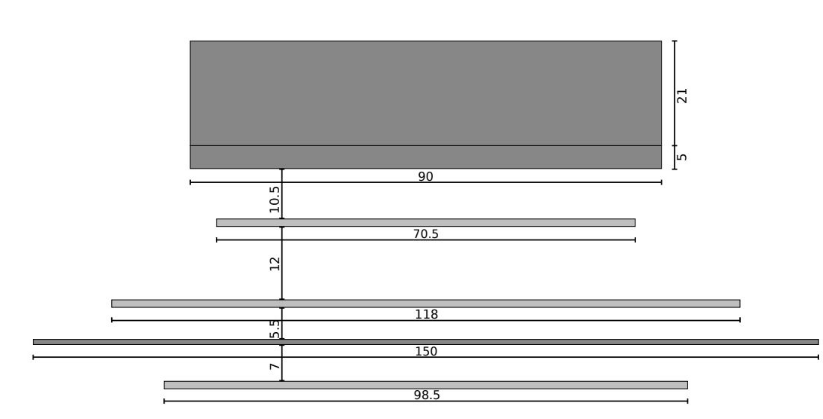
\includegraphics[width=0.63\textwidth]{figures/11.png}
		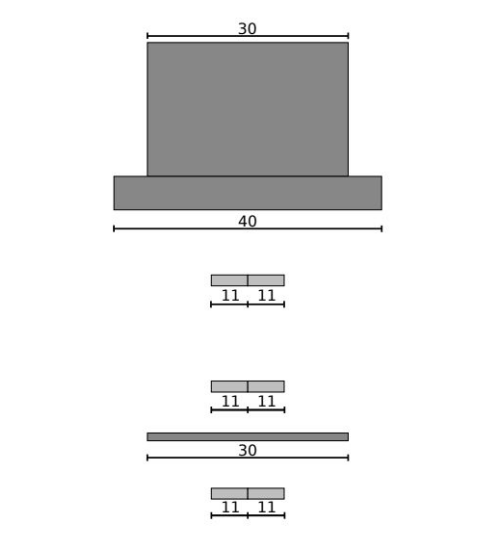
\includegraphics[width=0.36\textwidth]{figures/22.png}
		\caption{The experimental setup where it is shown in lateral and front view the absorber layers (dark grey) and the scintillator planes (light grey) with the dimensions in cm. Ref. Lab Manual Part 1}
		\label{fig:Scintillators_Detectors}
	\end{figure}
	\begin{figure}
		\centering
		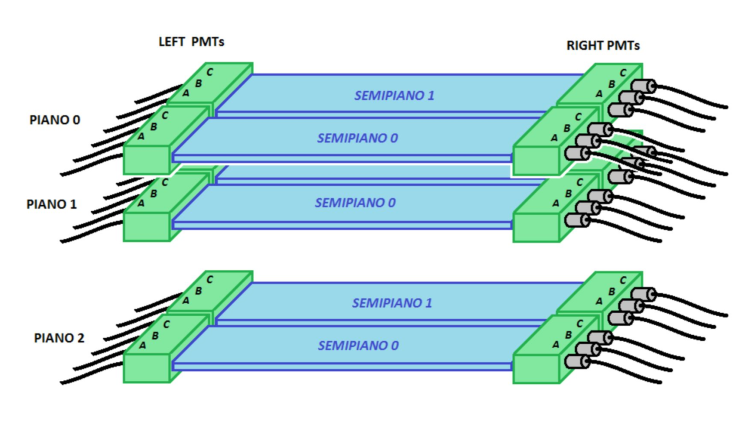
\includegraphics[width=1\textwidth]{figures/33.png}
		\caption{Scintillators with PMTs arranged in planes. Ref. Lab Manual Part 1}
		\label{fig:Setup}
	\end{figure}
	\vskip 0.09 cm
	Other than the detector itself, we use a NIM (Nuclear Instrument Modules) and a 
    CAMAC (Computer Automated Measurement And Control) crate with appropriate boards and modules.
    All algorithms and tunings of the experiment are done within the NIM crate and CAMAC is used
    for the read-out. The NIM modules which are used can be summarized as follows: 
	\vskip 0.09 cm
	\textbf{HV power supply:}\\ N470 CEAN 4 Channel NIM Programmable High Voltage
    Power Supply.\\
	This module is the power supply to the photomultiplier tubes.
	\vskip 0.09 cm
	\textbf{Discriminator:}\\ N840 CEAN 8 Channel Leading Edge Discriminator module; pulse width:
    5-40\,ns, and threshold 1-255\,mV.\\
	Given an analog input signal, the discriminator compares the amplitude with a threshold 
    (in mV since it is amplitude). If the falling edge of the input signals overcomes the threshold
    then a LOGIC 1 signal is produced as output. If the signal is lower than the threshold,
    a LOGIC 0 is generated. The Standard LOGIC used by this module is the Nuclear Instrument
    Module Logic (NIM).
	\vskip 0.09 cm
	\textbf{Logic Unit}:\\ CAEN N405 3-fold logic unit module having 3 independent sections to
    perform logic AND/OR up to 4 logic signals in input.\\
	It provides 1 linear OUT (width of the signals depending on input signals superposition),
    2 fixed width (adjustable) OUT signals, 1 ANTI OUT signal, and 1 VETO input.\\
	The first signal enters the LOGIC unit. During this time it is “1” the other signal arrives
    so there is $\Delta t$ during which both signals are “1”. 
    This means the signals coincide and an AND signal is produced.
	\vskip 0.09 cm
	\textbf{FI/FO}:\\ CAEN N625 Quad Linear FAN-IN FAN-OUT module\\
	The module has 4 identical sections. Each section has 4 inputs that can be fed with analog
    signals. Then for each section, there are 4 identical OUT signals. If only one IN is used the
    4 OUT are the replica of the IN signal. If more than one IN is connected then the OUTs provide
    the sum of the IN signals. So each of the 4 sections of this module can be used to replicate 
    a signal 4 times (4 OUT).
	\vskip 0.09 cm
	\textbf{Counter/Scaler:}\\ CAEN N1145 Quad Scaler and Preset Counter/Timer\\
	Count 4 NIM or TTL level signals for a given time interval defined by the user.
    The user can follow the countdown and read the number of counts on displays.
    	\vskip 0.09 cm
	\textbf{Dual Timer:}// CEAN N93B Dual Timer module//
	This NIM module housing two identical triggered pulse generators which produce NIM and ECL pulses whose width ranges from 50 ns to 10 s when 	triggered. Output pulses are provided normal and complementary. Timers can be re-triggered with the pulse end marker signal.
	
	\vskip 0.09 cm
	\textbf{Dual Delay:}// CEAN N108A Dula delay module//
	Delay ranges from 0 to 63.5 ns (+ 1.6 ns offset) per section. The delay can be set in 0.5 ns steps. The delay lines are made up of calibrated coaxial cable stubs for high accuracy delay and do not require power supply.
	
	\vskip 0.09 cm
	\textbf{Oscilloscope:}//
	
	\vskip 0.09 cm
	\textbf{TDC:}// CAEN mod. C414\\
	A single width CAMAC unit housing 8 independent 12 bit time-to-digital conversion channels. The full scale time can be selected from 100 ns to 5 μs via internal DIP switches. The time resolution ranges from 25 ps to 1.25 ns (respectively for 100 ns and 5 μs full scale time range). The conversion time is 2.5 μs per channel and it is reduced to 1.5 μs for overflow channels. A CAMAC LAM is generated (if enabled) at the end of the conversion.
